\documentclass[11pt,a4paper]{report}

\usepackage{lmodern}
\usepackage{amsmath, amsfonts}

\usepackage{tikz}

\usepackage{graphicx}
\graphicspath{{./fig/}}

\usepackage[svgpath=fig/]{svg}

\begin{document}
 \title{  Automatic Speech Recognition for PR2 Robotic Control under ROS   } 
\author{Weipeng He, Natalia Orlova}
\date{\small Report in Masterproject Intelligent Robotics, WS 2013/2014\\
Department of Informatik\\ Hamburg University\\[4mm]
\today }
\maketitle

\begin{abstract}
  In this report we would like to present the theories and implementations of our speech recognition system on PR2. 
\end{abstract}

\tableofcontents

\listoffigures

\chapter{Introduction}

\chapter{Speech Processing Basics}

\section{Implementation of Audio I/O System}
Although there are plenty of literatures about the theories of audio processing, there rarely are detailed documents on how the systems are implemented. To close the gap between theories and implementation, in this section, we would like to address the basic concepts of audio programming as well as details of the implementation of basic audio input and output in our system.

Theories of audio processing are always seemed to be neat and appealing. However, when it comes to writing a program to realize an algorithm, much more ``dirty'' works will be involved. These extra works are largely due to handling of hardware status and numerical computing, which are sometimes neglected in theories.

In this section, we will first introduce the basic concepts of digital audio signal processing. Afterward, we will show how to implement a minimal audio recording program using the Advanced Linux Sound Architecture (ALSA).

\subsection{Sampling and PCM}
To process an audio signal, first of all, we need to know how the signal is represented. Ideally, the audio signal is just amplitudes over time (time-domain signal), namely $ x(t) \in \mathbb{R},~ t \in \mathbb{R} $. However, practically, we need to represent the signal discretely. Thus, discretization on both time and amplitude (\textit{sampling} and \textit{quantization}, respectively) should be applied. As the result, the signal is represented using a sequence of quantized values $x_n$.

For sampling, we take the values of the continuous signal using a \textit{sampler} at $T_s$ time intervals: \[ x_s[n] = x(n T_c) \in \mathbb{R},~ n \in \mathbb{Z} \] Here, $T_s$ is called the \textit{sampling period}, and $ f_s = \frac{1}{T_c} $ is called the \textit{sampling frequency}.

After sampling, the \textit{A/D converter} converts the real values to a limited set of values, which can be represented by binary data. In digital audio, \textit{Pulse-code modulation} (PCM) is the most common method for this quantization process. 

\begin{figure}[htbp]
  \centering
  \input{fig/samquan}
  \caption{Sampling and Quantization of Audio Signal.}
  \label{fig:sqas}
\end{figure}

PCM has several quantization methods, which includes Linear PCM, A-law algorithm or $\mu$-law algorithm. Although different algorithms exist, PCM sometimes refer to Linear PCM by default as it is the most popular. Linear PCM quantize each sample using linearly uniform levels. In other words, all adjacent levels have the same difference in sound amplitude. The number of levels depends on the bit depth of each code.

Within each quantization method, different encoding method, e.g. \textit{format}, can be chosen. These formats are named according to the bit depth, endianness, float/integer and signed/unsigned that they use. For example, a format can be 32 bits signed integer with little endian. Some applications and libraries, such as aplay, ALSA, gstreamer, use a short name for each format. As for the example format, the name is ``\texttt{S32\_LE}''. The structure of the format name is shown in Figure \ref{fig:pcmname}. Other common formats includes \texttt{S8}, \texttt{U8}, \texttt{S16\_LE}, \texttt{F32\_LE}, \texttt{F64\_LE}, etc.

\begin{figure}[htpb]
\begin{center}
  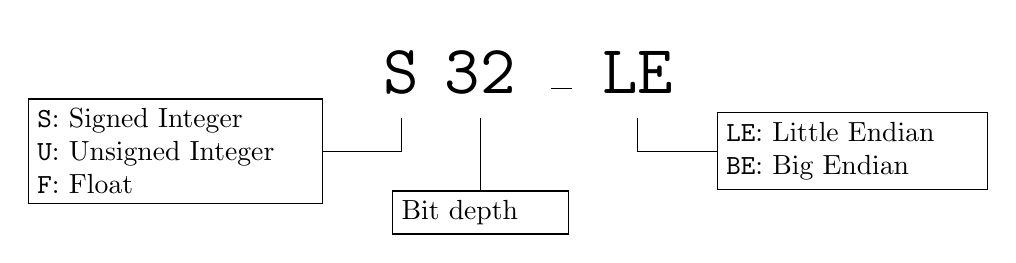
\begin{tikzpicture}
    {\Huge\texttt{
      \node(s) at (0,0) {S};
      \node(b) at (1,0) {32};
      \node at (2,-0.2) {\_};
      \node(e) at (3,0) {LE};
    }}
    \draw (-1,-1) node[left,text width=3.5cm,draw,rectangle]
       {\texttt{S}: Signed Integer\\\texttt{U}: Unsigned Integer\\\texttt{F}: Float} -| (s.south);
    \draw (1,-1.5) node[below,text width=2cm,draw,rectangle]
       {Bit depth} -- (b.south);
    \draw (4,-1) node[right,text width=3.2cm,draw,rectangle]
       {\texttt{LE}: Little Endian\\\texttt{BE}: Big Endian} -| (e.south);
  \end{tikzpicture}
\end{center}
\caption[Name structure of PCM format.]{Name structure of PCM format. The first letter represents the data type. Then follows a number, which is the bit depth of each sample. If the bit depth is larger than 8 (1 byte), then there is a tag, which states the endianness, at the end.}
  \label{fig:pcmname}
\end{figure}

Now, we can represent a single channeled audio recording using a sequence of PCM binary data. Furthermore, for multi-channeled audio recording, it it just simple interleave the data of each channel. A set of samples at one time from all channels is called a \textit{frame}. For example, suppose we have a 2-channeled data using \texttt{S16\_LE} format. Then the first 2 bytes are the first sample of channel 1, and the second 2 bytes are the first sample of channel 2. Thus, bytes number 1 to 4, are the first frame. And, the second samples of both channels are at the number 5 to 8 bytes, which consist the second frame. And so on.

To summarize, an audio recording can be represented by binary data using PCM. To sufficiently understand how the audio are encoded, we need to know the following parameters: sampling rate, number of channels and PCM format.

\subsection{Advanced Linux Sound Architecture}
Advanced Linux Sound Architecture (ALSA) is the software framework that provides API for sound device drivers as part of the linux kernel. The API includes configuration of the hardware and write/read audio data.

Besides the aforementioned parameters for audio representation (sampling rate, number of channels and PCM format), some other parameters regarding the hardware buffer are also need to be configured. These parameters are period size and buffer size. As it could be very costly for CPU to fetch the data one sample at a time, normally there is a hardware interrupt every interval. The number of frames that is in this interval is called the \textit{period size}. These data are stored in a ring buffer, and its size if called \textit{buffer size}. Usually the buffer size is twice as the period size. However, it can sometimes be up to 8 times of that.

% \subsection{Implementation using ALSA}

\section{Short Time Fourier Transform}
In previous section, we introduced the basics about speech signal in time domain. However, it can be difficult to analyze the time-domain signal. By using Fourier transform, we can change the signal to frequency domain and benefit from its several properties. Still, the problem for Fourier transform is that the speech signal is quasi-stationary (slowly varying over time) rather than stationary. Which means frequency-domain signal cannot specify the local information at a specific time. Therefore, the \textit{Short Time Fourier Transform} (STFT) is applied, in order to modeling the signal in both time and frequency domains.

\subsection{Window Function}
In STFT, the idea of ``short time'' is realized by applying a window function to the original signal at a specific time. Window function is zero-centered and non-zero in only a short interval. Typical window functions include: Hann window, Hamming window\cite{heinzel_spectrum_2002}. The Hann window (Figure \ref{fig:hann}) is defined as:
\[ w(n) = 0.5 (1 - \cos(\frac{2\pi n}{N-1})) \]
and Hamming window (Figure \ref{fig:hamming}) is defined as:
\[ w(n) = \alpha - \beta \cos(\frac{2\pi n}{N-1}) \]
where $\alpha = 0.54, \beta = 1 - \alpha = 0.46$ and $N$ is the window size.

\begin{figure}[htbp]
  \centering
  {\small
  \includesvg[pretex=\footnotesize,width=.8\textwidth]{hann}
  }
  \caption[Hann Window]{Hann Window.}
  \label{fig:hann}
\end{figure}

\begin{figure}[htbp]
  \centering
  {\small
  \includesvg[pretex=\footnotesize,width=.8\textwidth]{hamming}
  }
  \caption[Hamming Window]{Hamming Window.}
  \label{fig:hamming}
\end{figure}

\subsection{Continuous STFT and its Inverse}
Continuous STFT is simply traditional Fourier transform applied to windowed signal. Mathematically, continuous STFT is expressed as:
\[ X(\tau, \omega) = \mathcal{F}(x(t)w(t-\tau)) =  \int_{-\infty}^{\infty} x(t)w(t-\tau)e^{-j\omega t}\mathrm{d}t \]
where $\mathcal{F}$ is the Fourier transform, $x(t)$ is the time-domain signal to be transfered and $w(t)$ is the window function. For a fixed time $\tau$, $x(t)w(t-\tau)$ is just the original signal at local time around $\tau$ and masked by the window function. Thus, $X(\tau, \omega)$ represents the frequency attributes at that local time. We can also notice that the transform $X(\tau, \omega)$ depends on both time $\tau$ and frequency $\omega$. Therefore, we say that this kind of representation the time-frequency representation.

Like Fourier transform, the continuous STFT is invertible. Now we show how the inverse transform is derived. First, we assume the window function is scaled to have $\int_{-\infty}^{\infty} w(t) \mathrm{d}t = 1$. Thus:
\[
  x(t) = x(t) \int_{-\infty}^{\infty} w(t-\tau) \mathrm{d}\tau = \int_{-\infty}^{\infty} x(t)w(t-\tau) \mathrm{d}\tau
\]
The integrand $x(t)w(t-\tau)$ is actually the original signal of $X(\tau, \omega)$ before Fourier transform with $\tau$ fixed. Therefore:
\[ x(t)w(t-\tau) = \mathcal{F}^{-1}(X(\tau, \omega)) = \frac{1}{2\pi} \int_{-\infty}^{\infty} X(\tau, \omega) e^{j\omega t} \mathrm{d}\omega \]
Combining the two equations above, we have the inverse of the transform:
\[ x(t) = \frac{1}{2\pi} \int_{-\infty}^{\infty} \int_{-\infty}^{\infty} X(\tau, \omega) e^{j\omega t} \mathrm{d}\omega \mathrm{d}\tau \]

\subsection{Discrete STFT}
Because we don't have continuous speech signal, we shall extend the STFT to discrete situation\footnote{Most time, without specification, STFT means discrete STFT by default.}. Like the discrete Fourier transform (DFT), discrete STFT is defined as:
\[ X(n, k) = \sum_{m = -\infty}^{\infty} x[m]w[m-n]e^{-j \frac{2\pi k}{N} m} \]
where $x$ is the signal, $w$ is the window function, $n$ is the index of time, $k$ is the index of frequency bin, and $N$ is the number of frequency bins. Practically, most applications of STFT use Fast Fourier Transform to calculate. Thus, the $N$ is also equal to the window size and is an exponential of 2.

The magnitude squared of the STFT yields the spectrogram of the function:
\[ \text{Spectrogram}(n, k) = \left|X(n,k)\right|^2 \]
From the spectrogram we can clearly visualize the different frequency components of a sound and its variation over time. In fact, most application for extracting audio feature use only the magnitude information.

Note that because the time-domain signal is real, at any time, the result of the DFT has the following properties:
\begin{itemize}
  \item $X(n,0)$ and $X[n, \frac{N}{2}]$ are real;
  \item $X(n,k) = X^*(n,N-k), k \neq 0, \frac{N}{2}$, here $^*$ is the complex conjugate.
\end{itemize}
Therefore, only the first half (index from $0$ to $\frac{N}{2}$) of the DFT contains information, while the other half are redundant. In fact, only the first half is plotted in the spectrogram. From Fourier analysis theories, we know that the $k$th frequency bin represents the component at frequency $\frac{kf_s}{N}$, with $f_s$ is the sampling rate. The component with the highest frequency is the bin with index $\frac{N}{2}$ and its frequency is $\frac{N}{2} \times \frac{f_s}{N} = \frac{f_s}{2}$. This is consistent with the Nyquist frequency.

One shortcoming for STFT is that the frequency resolution and time resolution is mutually limited. This limit is referred as \textit{Gabor limit}. The difference of two consecutive frequency bin is $\frac{f_s}{N}$. And, one STFT is a DFT of a neighborhood of $N$ samples, e.g. $N * \frac{1}{f_s}$ time interval. That means the time resolution is $\frac{N}{f_s}$. Therefore, the product of the two resolutions, $\frac{f_s}{N} \times \frac{N}{f_s} = 1$, is constant. Selecting the windows size involves trade-off between the frequency resolution and time resolution. With large window size, we can have good frequency resolution, while it can be difficult to catch the change in a short time. Vice versa, with a small windows size, we can have high time resolution. However, the frequency resolution would be low.

\subsection{Inverse Discrete STFT}
Because DFT is invertible, calculating the inverse of STFT can be quite direct. For any $n$, we can find $m$, such that $w[n-m] \neq 0$. We have:
\[ x[n]w[n-m] = \mathcal{F}^{-1}(X(m,k))[n] \]
where $\mathcal{F}^{-1}$ is the inverse DFT. Thus,
\begin{equation}
  x[n] =  \frac{\mathcal{F}^{-1}(X(m,k))[n]}{w[n-m]} = \frac{\frac{1}{N}\sum_{k=0}^{N-1} X(m,k)e^{j \frac{2\pi k}{N} n}}{w[n-m]}
  \label{eq:naiveinv}
\end{equation}

We can clearly see that there could be multiple $m$, which yields the same result. In other words, the STFT is redundant. Therefore, except for calculating every $n$, we jump a interval between calculation of DFT. Which means, we use a shifting window, that shift more than 1 sample a time. With the \textit{shift size} $L$, we calculate the STFT at time $0$, $L$, $2L$, \dots. Thus, we can have windows that covers $[0, N-1]$, $[L, L+N-1]$, $[2L, 2L+N-1]$, \dots. In order to cover all samples, we need $L<N$, which means we have overlapping windows. Normally, we choose $L = \frac{N}{2}$ or $L = \frac{N}{4}$.

Although Equation \ref{eq:naiveinv} can still be used for calculating the inverse, it is not a good practice. It is because the $w[n-m]$ in the denominator can be very small, which amplifies small perturbation in the STFT. One of the algorithms to solve this issue is called the \textit{Overlap-add} (OLA) method.

The idea of OLA is simply calculating the inverse of all window frames and take the weighted average of them. The inverse is calculated as:
\begin{equation}
  x[n] = \frac{\sum_{p=-\infty}^{\infty} \mathcal{F}^{-1}(X(pL,k))[n]}{\sum_{p=-\infty}^{\infty} w[n-pL]}
  = \frac{\sum_{p=-\infty}^{\infty} \sum_{k=0}^{N-1} X(pL,k)e^{j \frac{2\pi k}{N} n}}{N\sum_{p=-\infty}^{\infty} w[n-pL]}
\end{equation}

Under some constraint, $\sum_{p=-\infty}^{\infty} w[n-pL] = W_0$ is constant. Then the inverse STFT is:
\begin{equation}
  x[n] = \frac{1}{NW_0} \sum_{p=-\infty}^{\infty} \sum_{k=0}^{N-1} X(pL,k)e^{j \frac{2\pi k}{N} n} 
  \label{eq:olainv}
\end{equation}



\chapter{Sound Source Separation}

\chapter{Noise Reduction Techniques}

\chapter{Conclusion}


\bibliographystyle{plain}
\bibliography{project}
 
\end{document}
